\begin{frame}[t]{Numerical example}
\begin{columns}[T] % align columns
\begin{column}{.48\textwidth}
We solve the following PDE problem:
\begin{subequations}
\begin{empheq}[left= \empheqlbrace]{align}
    \; -\nabla \cdot ( \nabla u) & = 0.21x^{-1.3} &  x \in (0,10), \notag \\
    u & = 0 &  x =0, \notag \\
    ( \nabla u) \cdot \bf{n}  & = 0.7x^{-0.3}  &  x=10. \notag 
\end{empheq}
\end{subequations}

Exact solution: $u_{exact}=x^{0.7}$.
\vspace{0.5cm}

Loss value of the exact solution: $\mathcal{L}_{\mathcal{R}}(u)=-1.54$.

\end{column}%

\hfill%

\begin{column}{.48\textwidth}
\begin{figure}[!htp]
\centering
 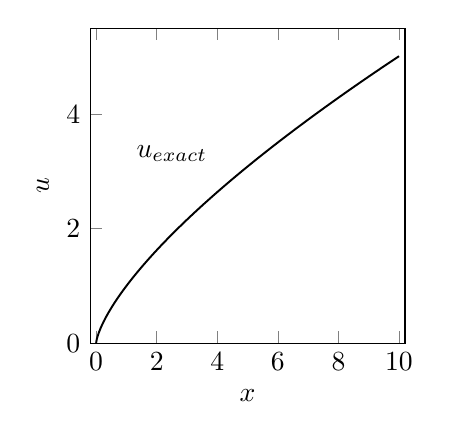
\begin{tikzpicture}
\begin{axis}[scale only axis, xlabel = $x$, ylabel = $u$, ytick pos=left, y label style={at={(-0.1,0.5)}}, legend style= {at={(0.6,0.98)},draw=none,fill=none,nodes={scale=0.8, transform shape}}, legend cell align={left}, height=4cm, width=4cm, xmin=-0.2, ymin=0, xmax=10.2, ymax=5.5,samples=1000]
\addlegendimage{only marks, mark=-, color=black} 
\addplot [black, line width=0.7pt,domain=0:10] {x^0.7};
%\addlegendentry{Exact solution}
% Legend
\node[anchor = south] at (2.5,3){\textcolor{black}{$u_{exact}$}};
\end{axis}
\end{tikzpicture}

%\caption*{Loss evolution.}
	\label{fig:ritz_exact}
 \end{figure}
\end{column}%
\end{columns}
\end{frame}


\begin{frame}[t]{Loss function}
Let $\{ K_i \}_{i=1}^{n}$ be a partition of $\Omega$ and $\{ L_j \}_{j=1}^{m}$ a partition of $\Gamma_N$.

\begin{equation}
\mathcal{L}_{\mathcal{R}}(u) = \frac{1}{2} \sum_{i=1}^{n} ( \nabla u,\nabla u)_{K_i} - \sum_{i=1}^{n} (f,u)_{K_i} - \sum_{j=1}^{m} (g,u)_{L_j}.
\notag
\end{equation}

\textbf{Gradient computation:}
\vspace{0.15cm}

\begin{itemize}
\item Automatic differentiation.
\end{itemize}

\vspace{0.25cm}
\textbf{Gaussian Quadrature:} Three Gaussian points.
\vspace{0.15cm}
\begin{figure}[!htp]
\centering
	\begin{tikzpicture}
\draw (0,0) -- (8,0);
\foreach \Point in {(0,0), (8,0)}{\node at \Point {\textbullet};}
\foreach \Point in {(1,0), (4,0), (7,0)}{\node[blue] at \Point {\textbullet};}
%\node at (9.5,0) {\textup{Training set}};
\node[blue] at (1,0.3) {$q_1$};
\node[blue] at (4,0.3) {$q_2$};
\node[blue] at (7,0.3) {$q_3$};
\node at (0,-0.25) {$x_i$};
\node at (8,-0.25) {$x_{i+1}$};
\end{tikzpicture}
	\label{fig:partition}
\end{figure} 
\end{frame}


\begin{frame}{Architecture Sketch}
\def\layersep{1.5cm}
\centering

%\begin{tikzpicture}[x=1cm,y=0.8cm]
%%\draw[very thin, rounded corners=5pt,fill=orange!30!white ,opacity=0.5] (4.0,0.2) rectangle (10,1.3);
%\node at (7.0,0.75){\Large $u \approx u_{NN} := \underset{\theta \in V}{\textup{ arg min }} \mathcal{L}_{(\cdot)}(\theta)$};
%\end{tikzpicture}
%
%\vspace{0.4cm}

\begin{tikzpicture}[shorten >=1pt,->,draw=black!50, node distance=\layersep]
    \tikzstyle{every pin edge}=[<-,shorten <=1pt]
    \tikzstyle{neuron}=[circle,fill=black!25,minimum size=20pt,inner sep=0pt]
    \tikzstyle{neuron2}=[circle,fill=black!25,minimum size=15pt,inner sep=0pt]
    \tikzstyle{input lay}=[rectangle,fill=green!50,minimum width=30pt, minimum height=100pt,inner sep=0pt]
%    \tikzstyle{input neuron}=[neuron, fill=green!50];
	\tikzstyle{hidden neuron}=[neuron2, fill=blue!50];
	\tikzstyle{ghost neuron}=[neuron, fill=gray!40!white, , opacity=1];
    \tikzstyle{output neuron}=[neuron, fill=red!50];
    \tikzstyle{output lay}=[rectangle,fill=red!50,minimum width=30pt, minimum height=100pt,inner sep=0pt]
    
	\tikzstyle{multi neuron}=[neuron, fill=purple!50];
    \tikzstyle{multi lay}=[rectangle,fill=purple!50,minimum width=30pt, minimum height=100pt,inner sep=0pt]	
	
	
	\tikzstyle{final neuron}=[neuron, fill=brown!50];
	
    \tikzstyle{annot} = [text width=4em, text centered]
	\tikzstyle{annot final} = [text width=10em, text centered]


\draw[very thin, rounded corners=5pt,fill=gray!40!white ,opacity=1] (0,1.5) rectangle (6,-4);
\draw[very thin, rounded corners=5pt,fill=gray!30!white ,opacity=1] (0.3,1.8) rectangle (4.0,1.2);
\node [anchor = west] at (0.3,1.5){Deep Neural Network};

    % Draw the input layer nodes
    \foreach \name / \y in {1}
        \node[input lay] (I-\name) at (0,-1) {$x$};

%    % Draw the hidden layer nodes
%    \foreach \name / \y in {1,...,3}
%        \path[yshift=1.5cm]
%            node[hidden neuron, xshift=0.5cm] (H-\name) at (\layersep,-\y cm) {};
	
\path[yshift=1.5cm] node[hidden neuron, xshift=0.5cm] (H1_1) at (\layersep,-1 cm) {};	
\path[yshift=1.5cm] node[hidden neuron, xshift=0.5cm] (H1_2) at (\layersep,-2 cm) {};
\path[yshift=1.5cm] node[ghost neuron, xshift=0.5cm] (Hghost1) at (\layersep,-3 cm) {$\vdots$};
\path[yshift=1.5cm] node[hidden neuron, xshift=0.5cm] (H1_3) at (\layersep,-4 cm) {};
	
\path[yshift=1.5cm] node[hidden neuron, xshift=0.0cm] (H2_1) at (2.5*\layersep,-1 cm) {};	
\path[yshift=1.5cm] node[hidden neuron, xshift=0.0cm] (H2_2) at (2.5*\layersep,-2 cm) {};
\path[yshift=1.5cm] node[ghost neuron, xshift=0.0cm] (Hghost2) at (2.5*\layersep,-3 cm) {$\vdots$};
\path[yshift=1.5cm] node[hidden neuron, xshift=0.0cm] (H2_3) at (2.5*\layersep,-4 cm) {};

\path[yshift=1.5cm] node[ghost neuron, xshift=0.2cm] (Hghosta) at (1.75*\layersep,-1 cm) {$\hdots$};
\path[yshift=1.5cm] node[ghost neuron, xshift=0.2cm] (Hghostb) at (1.75*\layersep,-2 cm) {$\hdots$};
\path[yshift=1.5cm] node[ghost neuron, xshift=0.2cm] (Hghostc) at (1.75*\layersep,-4 cm) {$\hdots$};

%    % Draw the output layer node
    \node[output lay, right of=Hghost2, yshift=0.5cm, xshift=0.5cm] (O) {$\tilde{u}_{NN, \theta}$};
    
    % Multiply BC function
	\node[multi lay, right of=O,  xshift=1.5cm] (M) {$u_{NN, \theta}$};
%	\node[multi lay, right of=Hghost2, yshift=0.5cm, xshift=0.5cm] (M) {$u_{NN}$};
	
	% Final output, after Loss
	\node[final neuron, right of=M, xshift=1.8cm] (F) {$\mathcal{L}(u_{NN, \theta})$};

    % Connect every node in the input layer with every node in the
    % hidden layer.
    \foreach \source in {1}
        \foreach \dest in {1,...,3}
            \path (I-\source) edge (H1_\dest);

    % Connect every node in the hidden layer with the output layer
    \foreach \source in {1,...,3}
        \path (H2_\source) edge (O);
        
%	% Connect output kayer and multiply layer
	\path[every node/.style={anchor=south}] (O) edge node {Impose BC} (M);
	
	% Connect output kayer and multiply layer
	\path[every node/.style={anchor=south}] (M) edge node {Define loss} (F);

    % Annotate the layers
%    \node[text width=10em, text centered, ,above of=Hghosta, node distance=0.7cm] {Hidden layers};
    \node (texto)[text width=15.5em, text centered, ,below of=Hghostc, node distance=1cm] {Trainable parameters: \\ $\theta:= \{$weights, biases$\}$};
    
%    \node[text width=6.5em, text centered, ,right of=texto, node distance=4.5cm] {Non-trainable layer};
%    \node[text width=6.5em, text centered, ,right of=texto, node distance=7.5cm] {Non-trainable layer};
    
%    \node[text width=4em, text centered, ,above of=I-1, node distance=2.cm] {\footnotesize INPUT};
%    \node[text width=4em, text centered, ,above of=F, node distance=1.cm] {\footnotesize OUTPUT};
\end{tikzpicture}

\vspace{0.2cm}
\small To impose the homogeneous Dirichlet BC, we define:

$u_{NN, \theta} := \phi(x) \cdot \tilde{u}_{NN, \theta}$, where 
$ \left\{
\begin{array}{l}
\phi(x) = 0,  \quad \text{if} \; x \in \Gamma_D,\\ 
\phi(x) \neq 0, \quad \text{if} \; x \not \in \Gamma_D.
\end{array}
\right.$
\end{frame}


\begin{frame}[t]{Numerical example}
\visible<1-2>{Loss evolution of the DL method optimization process.

\begin{figure}[!htp]
\centering
 \begin{tikzpicture}
%https://tex.stackexchange.com/questions/451704/tikz-position-of-an-imported-image
  \node[anchor=south west,inner sep=0] (image) at (0,0) {\begin{tikzpicture}
\begin{axis}[scale only axis, xlabel = $Epoch$, ylabel = $Loss$, ytick pos=left, y label style={at={(-0.12,0.5)}}, legend style= {at={(0.65,0.35)},draw=none,fill=none,nodes={scale=0.8, transform shape}}, legend cell align={left}, height=4cm, width=12cm, xmin=0.95, ymin=-15, xmax=45000, ymax=12, ytick = {8,-1.54,-15}, xmode=log, xticklabel style={yshift=-3pt}, yticklabel style={xshift=-3pt}]
\addplot [black, dashed, line width=0.7pt,domain=0.99999:39900] {-1.54};
%\addlegendentry{Loss of exact solution}
\addplot[line width=0.8pt,color=red] %
	table[x=epoch ,y=loss]{Diapos/PDEs_with_NN/Figures/Quadrature_problem//Data//loss_Ritz_normal_treshold.csv};
%\addlegendentry{Loss of NN approximation};

\end{axis}
\end{tikzpicture}
};
  \begin{scope}[x={(image.south east)},y={(image.north west)}]
  \draw[<-] (0.3,0.55) -- (0.35,0.45) node[below right] {\textcolor{black}{$\mathcal{L}_{\mathcal{R}}(u_{exact})$}};
  \draw[<-, color=red] (0.35,0.7) -- (0.6,0.85) node[above right] {\textcolor{red}{$\mathcal{L}_{\mathcal{R}}(u_{NN})$}};
  \end{scope}
\end{tikzpicture}

%\caption*{Loss evolution.}
	\label{fig:ritz_normal_loss}
 \end{figure}}
 
\visible<2-2>{
\begin{center}
\textcolor{red}{We obtain a better loss than the optimum!}
\end{center}
}

\end{frame}


\begin{frame}[t]{Numerical example}
Mesh with four elements. Three Gauss points per element.
\vspace{0.5cm}

\begin{minipage}{.4\textwidth}
\begin{figure}[!htp]
\centering
 \begin{tikzpicture}
\begin{axis}[scale only axis, xlabel = $x$, ylabel = $u$, ytick pos=left, y label style={at={(-0.1,0.5)}}, legend style= {at={(0.6,0.98)},draw=none,fill=none,nodes={scale=0.8, transform shape}}, legend cell align={left}, height=4cm, width=4cm, xmin=-0.2, ymin=0, xmax=10.2, ymax=50]
\addlegendimage{only marks, mark=-, color=black} 
\addlegendimage{only marks, mark=-, color=red}
\addplot [black, line width=0.7pt,domain=0:10] {x^0.7};
%\addlegendentry{Exact solution}
\addplot[line width=0.5pt,color=red] %
	table[x=x ,y=u_pred]{Diapos/PDEs_with_NN/Figures/Quadrature_problem//Data//data_Ritz_normal.csv};
%\addlegendentry{Gauss/AD};
\addplot[densely dashed, blue] coordinates {
      (0.01, 18)
      (2.5, 18)
      (2.5,  48)
      (0.01, 48)
      (0.01, 18)
    };

% Legend
\node[anchor = south] (Ua)at (6,32){\textcolor{red}{$u_{NN}$}};
\node[anchor = south] at (6,6){\textcolor{black}{$u_{exact}$}};

\end{axis}
\end{tikzpicture}

\caption*{Exact and approximated solutions}
	\label{fig:ritz_exact}
 \end{figure}
\end{minipage}%
\begin{minipage}{.2\textwidth}
\center
\vspace{-2.5cm}
\tikzfancyarrow{Zoom}
\end{minipage}%
\begin{minipage}{.4\textwidth}
\begin{figure}[!htp]
\centering
 \begin{tikzpicture}
\begin{axis}[scale only axis, xlabel = $x$, ylabel = $u$, ytick pos=left, y label style={at={(-0.1,0.5)}}, height=4cm, width=4cm, xmin=0, ymin=18, xmax=2.5, ymax=50]
%\addlegendimage{only marks, mark=-, color=black} 
%\addlegendimage{only marks, mark=-, color=red}
\addplot [black, line width=0.7pt,domain=0:10] {x^0.7};
%\addlegendentry{Exact solution}
\addplot[line width=0.5pt,color=red] %
	table[x=x ,y=u_pred]{Diapos/PDEs_with_NN/Figures/Quadrature_problem//Data//data_Ritz_normal.csv};
\addplot[only marks, blue, mark size=1.25] coordinates {
      (0.28175, 19)
      (1.25, 46.27)
      (2.21825, 36.05)
    };
    


\node(G)[anchor = north, text width=1.0] at (axis cs: 1.5,30)
 {\textcolor{blue}{Gauss points}};
\node(G_aux1)[anchor = north, text width=1.0] at (axis cs: 1.65,31) {};
\node(G_aux2)[anchor = north, text width=1.0] at (axis cs: 2,31) {};
    

\node (G1) at (axis cs: 0.28175, 19){};
\node (G2) at (axis cs: 1.25, 46.27){};
\node (G3) at (axis cs: 2.21825, 36.05){};


\path[->, blue] (G) edge (G1);
\path[->, blue] (G_aux1) edge (G2);
\path[->, blue] (G_aux2) edge (G3);
%\addlegendentry{Gauss/AD};
\end{axis}
\end{tikzpicture}
\caption*{Zoom on the approximated solution}
	\label{fig:ritz_exact}
 \end{figure}
\end{minipage}%
\end{frame}


\begin{frame}[t]{Numerical example}
\begin{equation}
\notag
\mathcal{L}_{\mathcal{R}}(u_{NN}) = \frac{1}{2} \underbrace{( \nabla u_{NN},\nabla u_{NN})}_{ \sum_{q_i} \omega_i (\nabla u_{NN})^2 \approx 0} - \underbrace{(f,u_{NN})}_{\infty} - (g,u_{NN})_{\Gamma_N} \simeq - \infty
\notag
\end{equation}

\begin{figure}[!htp]
\centering
	%\subcaptionbox{Approximated solution at interval $[0,2.5]$}
	{\begin{tikzpicture}
\begin{axis}[scale only axis, xlabel = $x$, ylabel = $u$, ytick pos=left, y label style={at={(-0.1,0.5)}}, height=4cm, width=4cm, xmin=0, ymin=18, xmax=2.5, ymax=50]
%\addlegendimage{only marks, mark=-, color=black} 
%\addlegendimage{only marks, mark=-, color=red}
\addplot [black, line width=0.7pt,domain=0:10] {x^0.7};
%\addlegendentry{Exact solution}
\addplot[line width=0.5pt,color=red] %
	table[x=x ,y=u_pred]{Diapos/PDEs_with_NN/Figures/Quadrature_problem//Data//data_Ritz_normal.csv};
\addplot[only marks, blue, mark size=1.25] coordinates {
      (0.28175, 19)
      (1.25, 46.27)
      (2.21825, 36.05)
    };
    


\node(G)[anchor = north, text width=1.0] at (axis cs: 1.5,30)
 {\textcolor{blue}{Gauss points}};
\node(G_aux1)[anchor = north, text width=1.0] at (axis cs: 1.65,31) {};
\node(G_aux2)[anchor = north, text width=1.0] at (axis cs: 2,31) {};
    

\node (G1) at (axis cs: 0.28175, 19){};
\node (G2) at (axis cs: 1.25, 46.27){};
\node (G3) at (axis cs: 2.21825, 36.05){};

\draw[] (G1) node[above, blue] {\footnotesize $q_1$};
\draw[] (G2) node[above, blue] {\footnotesize $q_2$};
\draw[] (G3) node[above, blue] {\footnotesize $q_3$};


\path[->, blue] (G) edge (G1);
\path[->, blue] (G_aux1) edge (G2);
\path[->, blue] (G_aux2) edge (G3);
%\addlegendentry{Gauss/AD};
\end{axis}
\end{tikzpicture}} 
	\hspace{0.5cm}
	%\subcaptionbox{Loss evolution}
	{\begin{tikzpicture}
\begin{axis}[scale only axis, xlabel = $Epoch$, ylabel = $Loss$, ytick pos=left, y label style={at={(-0.25,0.5)}}, legend style= {at={(0.8,0.4)},draw=none,fill=none,nodes={scale=0.7, transform shape}}, legend cell align={left}, height=4cm, width=6cm, xmin=0.95, ymin=-15, xmax=45000, ymax=12, ytick = {8,-1.54,-15}, xmode=log]
\addplot [black, dashed, line width=0.7pt,domain=0.99999:39900] {-1.54};
%\addlegendentry{Loss of exact solution}
\addplot[line width=0.8pt,color=red] %
	table[x=epoch ,y=loss]{Diapos/PDEs_with_NN/Figures/Quadrature_problem//Data//loss_Ritz_normal_treshold.csv};
%\addlegendentry{Loss of NN approximation.};

% Legend
%\node[anchor = south] (Ua)at (6,32){\textcolor{red}{$u_{approx}$}};
%\node[anchor = south] at (6,6){\textcolor{black}{$u_{exact}$}};

\end{axis}
\end{tikzpicture}
}
\end{figure} 
\end{frame}

